\documentclass{article}
\usepackage[margin=0.75in]{geometry}
\usepackage[utf8]{inputenc}
\usepackage{amsmath}
\usepackage{amssymb}
\usepackage{graphicx}
\usepackage{hyperref}

\title{CORDIC Algorithm: Theory and Implementation}
\author{Antigravity AI Assistant}
\date{\today}

\begin{document}

\maketitle

\section{Introduction}
CORDIC (COordinate Rotation Digital Computer) is an algorithm to calculate trigonometric, hyperbolic, and other mathematical functions using only shifts and additions.

\subsection{Main Uses}
The primary applications of the CORDIC algorithm include:
\begin{itemize}
    \item Realization of rotations.
    \item Calculation of trigonometric functions ($\sin, \cos$) and inverse trigonometric functions ($\tan^{-1}(a/b)$).
    \item Calculation of magnitude ($\sqrt{a^2 + b^2}$).
    \item Extension to hyperbolic functions, natural logarithms, and exponentials.
    \item Division and multiplication.
    \item Pervasive use in DSP, Image Processing, 3D Graphics, and Robotics.
\end{itemize}

\section{The Core Idea: Successive Rotations}
A perfect rotation of a vector $(x_{in}, y_{in})$ by an angle $\theta$ results in $(x_R, y_R)$ given by:
\begin{align}
    x_R &= M_{in} \cos(\beta + \theta) = x_{in} \cos \theta - y_{in} \sin \theta \\
    y_R &= M_{in} \sin(\beta + \theta) = x_{in} \sin \theta + y_{in} \cos \theta
\end{align}
where $M_{in}$ is the modulus and $\beta$ is the initial angle. In matrix form:
\begin{equation}
    \begin{bmatrix} x_R \\ y_R \end{bmatrix} = \begin{bmatrix} \cos \theta & -\sin \theta \\ \sin \theta & \cos \theta \end{bmatrix} \begin{bmatrix} x_{in} \\ y_{in} \end{bmatrix} = \text{ROT}(\theta) \begin{bmatrix} x_{in} \\ y_{in} \end{bmatrix}
\end{equation}

\subsection{Micro-Rotations and Simplifications}
The key idea is to decompose the angle $\theta$ into a sequence of known elementary micro-rotation angles $\alpha_j$:
\begin{equation}
    \theta = \sum_{j=0}^{\infty} \alpha_j \implies \text{ROT}(\theta) = \prod_{j=0}^{\infty} \text{ROT}(\alpha_j)
\end{equation}

To avoid multiplications, the rotation is decomposed into a \textit{scaling operation} and a \textit{rotation-extension}:
\begin{align}
    x_R[j + 1] &= \cos(\alpha_j)(x_R[j] - y_R[j]\tan(\alpha_j)) \\
    y_R[j + 1] &= \cos(\alpha_j)(y_R[j] + x_R[j]\tan(\alpha_j))
\end{align}

By choosing elementary angles $\alpha_j = \sigma_j \tan^{-1}(2^{-j})$ with $\sigma_j \in \{-1, 1\}$, the rotation-extension recurrence relies only on additions and shifts:
\begin{align}
    x[j + 1] &= x[j] - \sigma_j 2^{-j} y[j] \\
    y[j + 1] &= y[j] + \sigma_j 2^{-j} x[j] \\
    z[j + 1] &= z[j] - \sigma_j \tan^{-1}(2^{-j})
\end{align}

\begin{figure}[h]
    \centering
    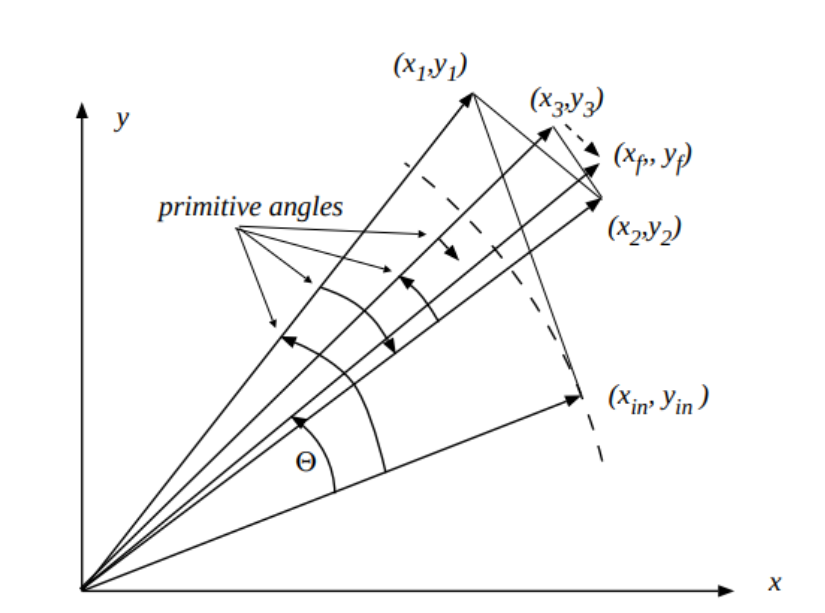
\includegraphics[width=0.6\textwidth]{cordic_microrotation_mode.png}
    \caption{Vector rotation using microrotations.}
    \label{fig:microrotation}
\end{figure}

\subsection{Scaling Factor Compensation}
The rotation-extension scales the modulus by $M[j+1] = \sqrt{1+2^{-2j}} M[j]$. The total scaling factor after $\infty$ iterations converges to a constant, independent of the target angle:
\begin{equation}
    K = \prod_{j=0}^{\infty} (1 + 2^{-2j})^{1/2} \approx 1.6468
\end{equation}

To compute true rotations, this scaling factor must be compensated. Common methods include:
\begin{itemize}
    \item \textbf{Direct Multiplication}: Multiply the final results by $1/K \approx 0.60725$.
    \item \textbf{Scaling Iterations}: Applying steps of the form $x_s = x \pm x \cdot 2^{-i}$.
    \item \textbf{Repeated Iterations}: Repeating certain CORDIC iterations to force the product to reach a known power of two or a stable target. For $n=24$, repetitions include iterations 1, 3, 5, 6.
\end{itemize}

\section{Unified Description}
The CORDIC algorithm can be generalized to three coordinate systems using a parameter $m$:
\begin{itemize}
    \item Circular ($m=1$)
    \item Linear ($m=0$)
    \item Hyperbolic ($m=-1$)
\end{itemize}

The unified microrotation is defined as:
\begin{align}
    x[j + 1] &= x[j] - m \sigma_j 2^{-j} y[j] \\
    y[j + 1] &= y[j] + \sigma_j 2^{-j} x[j] \\
    z[j + 1] &= 
    \begin{cases} 
        z[j] - \sigma_j \tan^{-1}(2^{-j}) & \text{if } m = 1 \\ 
        z[j] - \sigma_j \tanh^{-1}(2^{-j}) & \text{if } m = -1 \\ 
        z[j] - \sigma_j(2^{-j}) & \text{if } m = 0 
    \end{cases}
\end{align}
The specific initial values and rotation/vectoring mode outputs vary according to the coordinate system. Note that hyperbolic CORDIC ($m=-1$) must begin at $j=1$ (since $\tanh^{-1}(2^0) = \infty$) and requires specific iterations (e.g., 4, 13, 40) to be repeated to guarantee convergence.

\section{Operating Modes (Circular, $m=1$)}

\subsection{Rotation Mode}
Used to rotate a vector by a specific angle $\theta$. We start with $z[0] = \theta$.
\begin{itemize}
    \item \textbf{Objective}: Reduce $z$ to 0. 
    \item \textbf{Decision}: $\sigma_j = \text{sign}(z[j])$.
    \item \textbf{Result}: $x_f = K(x_{in} \cos \theta - y_{in} \sin \theta)$, $y_f = K(x_{in} \sin \theta + y_{in} \cos \theta)$, $z_f = 0$.
\end{itemize}
\begin{figure}[h]
    \centering
    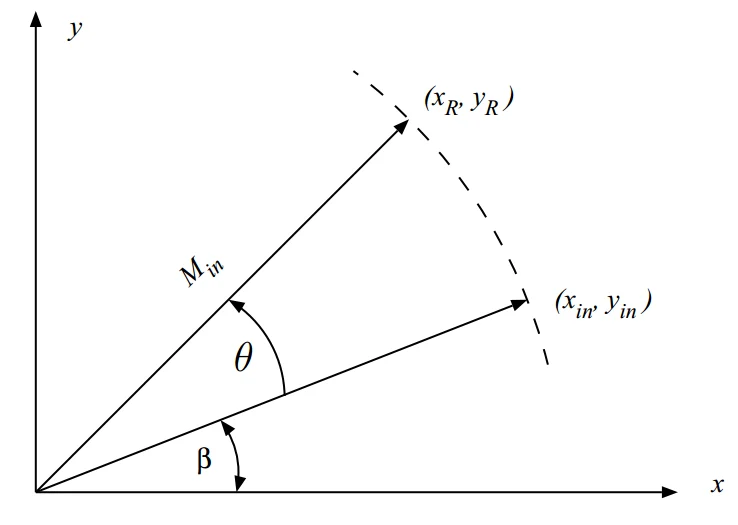
\includegraphics[width=0.45\textwidth]{cordic_rotation_mode.png}
    \caption{CORDIC Rotation Mode: Iteratively rotating a vector towards a target angle.}
\end{figure}

\subsection{Vectoring Mode}
Used to find the magnitude and angle (phase) of a vector $(x_{in}, y_{in})$.
\begin{itemize}
    \item \textbf{Objective}: Reduce $y$ to 0.
    \item \textbf{Decision}: $\sigma_j = -\text{sign}(y[j])$.
    \item \textbf{Result}: $x_f = K\sqrt{x_{in}^2 + y_{in}^2}$, $y_f = 0$, $z_f = z_{in} + \tan^{-1}(y_{in} / x_{in})$.
\end{itemize}
\begin{figure}[h]
    \centering
    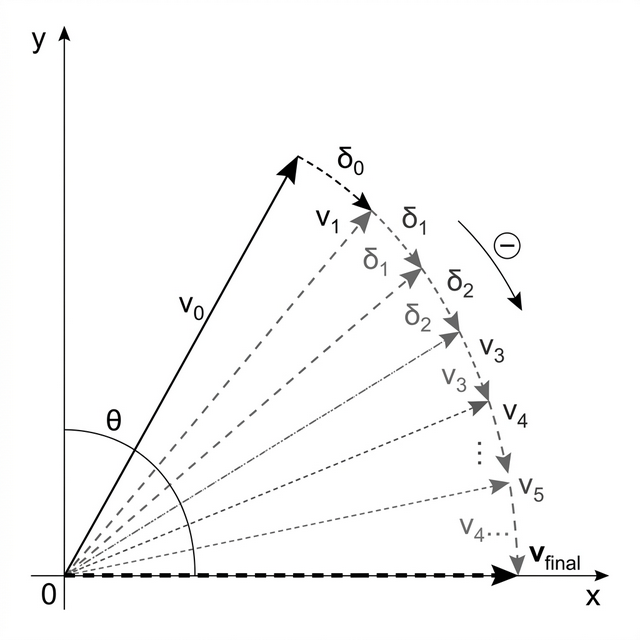
\includegraphics[width=0.45\textwidth]{cordic_vectoring_mode.png}
    \caption{CORDIC Vectoring Mode: Iteratively rotating an arbitrary vector towards the x-axis.}
\end{figure}


\section{Implementations}
CORDIC implementations generally fall into two architectural categories:
\begin{description}
    \item[Word-Serial] Hardware consisting of a single set of adders/subtractors and variable barrel shifters. The hardware is reused sequentially across $N$ clock cycles. This is resource-efficient but has lower throughput and requires routing multiplexers.
    \item[Pipelined] An unrolled hardware implementation with $N$ stages. Each stage corresponds to an iteration $j$ with hardwired shifts instead of barrel shifters. Highly efficient for streaming data (1 result per clock cycle after initial latency) but area-intensive.
\end{description}

\section{Redundant Representation and High Radix}
The critical path in a standard CORDIC implementation is the Carry-Propagate Adder (CPA) used to update $x, y, z$. To reduce this delay, redundant representation adders (e.g., carry-save) can be used.

However, redundant additions make strict sign evaluation difficult. If we use a redundant representation for $z$ (or $y$), calculating $\sigma_j = \text{sign}(z[j])$ precisely is impossible without a fast CPA. One solution is to allow $\sigma_j \in \{-1, 0, 1\}$ based on an estimate. 
If $\sigma_j = 0$, however, the scaling factor $(1 + 0 \cdot 2^{-2j})^{1/2} = 1$, which makes the final $K$ variable depending on the input data.

\subsection{Double Rotation Approach}
To retain redundant arithmetic without variable scaling factors, the Double Rotation approach forces two identical rotations unconditionally. For each iteration step $(j)$:
\begin{itemize}
    \item If $\sigma_j = 1$, rotate by $\tan^{-1}(2^{-(j+1)})$ twice.
    \item If $\sigma_j = -1$, rotate by $-\tan^{-1}(2^{-(j+1)})$ twice.
    \item If $\sigma_j = 0$, rotate by $\tan^{-1}(2^{-(j+1)})$ and then $-\tan^{-1}(2^{-(j+1)})$.
\end{itemize}
This ensures that regardless of $\sigma_j$, the scaling magnitude applied during step $j$ is strictly $1+2^{-2j-2}$, maintaining a constant $K$. The updated unified recurrence involves $q_j$ and $p_j$ terms determined by $\sigma_j$, requiring three-operand addition instead of two.

\end{document}
